% Options for packages loaded elsewhere
% Options for packages loaded elsewhere
\PassOptionsToPackage{unicode}{hyperref}
\PassOptionsToPackage{hyphens}{url}
\PassOptionsToPackage{dvipsnames,svgnames,x11names}{xcolor}
%
\documentclass[
  10pt,
  letterpaper,
  DIV=11,
  numbers=noendperiod]{scrartcl}
\usepackage{xcolor}
\usepackage{amsmath,amssymb}
\setcounter{secnumdepth}{5}
\usepackage{iftex}
\ifPDFTeX
  \usepackage[T1]{fontenc}
  \usepackage[utf8]{inputenc}
  \usepackage{textcomp} % provide euro and other symbols
\else % if luatex or xetex
  \usepackage{unicode-math} % this also loads fontspec
  \defaultfontfeatures{Scale=MatchLowercase}
  \defaultfontfeatures[\rmfamily]{Ligatures=TeX,Scale=1}
\fi
\usepackage{lmodern}
\ifPDFTeX\else
  % xetex/luatex font selection
\fi
% Use upquote if available, for straight quotes in verbatim environments
\IfFileExists{upquote.sty}{\usepackage{upquote}}{}
\IfFileExists{microtype.sty}{% use microtype if available
  \usepackage[]{microtype}
  \UseMicrotypeSet[protrusion]{basicmath} % disable protrusion for tt fonts
}{}
% Make \paragraph and \subparagraph free-standing
\makeatletter
\ifx\paragraph\undefined\else
  \let\oldparagraph\paragraph
  \renewcommand{\paragraph}{
    \@ifstar
      \xxxParagraphStar
      \xxxParagraphNoStar
  }
  \newcommand{\xxxParagraphStar}[1]{\oldparagraph*{#1}\mbox{}}
  \newcommand{\xxxParagraphNoStar}[1]{\oldparagraph{#1}\mbox{}}
\fi
\ifx\subparagraph\undefined\else
  \let\oldsubparagraph\subparagraph
  \renewcommand{\subparagraph}{
    \@ifstar
      \xxxSubParagraphStar
      \xxxSubParagraphNoStar
  }
  \newcommand{\xxxSubParagraphStar}[1]{\oldsubparagraph*{#1}\mbox{}}
  \newcommand{\xxxSubParagraphNoStar}[1]{\oldsubparagraph{#1}\mbox{}}
\fi
\makeatother


\usepackage{longtable,booktabs,array}
\usepackage{calc} % for calculating minipage widths
% Correct order of tables after \paragraph or \subparagraph
\usepackage{etoolbox}
\makeatletter
\patchcmd\longtable{\par}{\if@noskipsec\mbox{}\fi\par}{}{}
\makeatother
% Allow footnotes in longtable head/foot
\IfFileExists{footnotehyper.sty}{\usepackage{footnotehyper}}{\usepackage{footnote}}
\makesavenoteenv{longtable}
\usepackage{graphicx}
\makeatletter
\newsavebox\pandoc@box
\newcommand*\pandocbounded[1]{% scales image to fit in text height/width
  \sbox\pandoc@box{#1}%
  \Gscale@div\@tempa{\textheight}{\dimexpr\ht\pandoc@box+\dp\pandoc@box\relax}%
  \Gscale@div\@tempb{\linewidth}{\wd\pandoc@box}%
  \ifdim\@tempb\p@<\@tempa\p@\let\@tempa\@tempb\fi% select the smaller of both
  \ifdim\@tempa\p@<\p@\scalebox{\@tempa}{\usebox\pandoc@box}%
  \else\usebox{\pandoc@box}%
  \fi%
}
% Set default figure placement to htbp
\def\fps@figure{htbp}
\makeatother





\setlength{\emergencystretch}{3em} % prevent overfull lines

\providecommand{\tightlist}{%
  \setlength{\itemsep}{0pt}\setlength{\parskip}{0pt}}



 


\usepackage{xcolor, soul}
\definecolor{Light}{gray}{.90}
\sethlcolor{Light}
\let\OldTexttt\texttt
\renewcommand{\texttt}[1]{\OldTexttt{\hl{#1}}}
\usepackage{caption}
\captionsetup{font=small, labelfont=bf}
\setlength{\parindent}{0pt}
\setlength{\parskip}{1.25ex}
% Symbols %%%%%%%%%%%%%%%%%%%%%%%%%%%%%%%%%%%%%%%%%%%%%%%%%%%%%

\usepackage{amsthm}
\usepackage{amsmath}
\usepackage{amssymb}
\usepackage{amsfonts}

% New commands %%%%%%%%%%%%%%%%%%%%%%%%%%%%%%%%%%%%%%%%%%%%%%%%

% General mathematical symbols
% argmin help from egreg from tex.stackexchange.com/questions/5223
\newcommand{\R}{\mathbb{R}}
\newcommand{\onedim}{\mathbb{R}}
\newcommand{\ddim}{\mathbb{R}^d}
\newcommand{\kdim}{\mathbb{R}^k}

\newcommand{\eps}{\varepsilon}
\newcommand{\seq}[1]{\{ #1_{n} \}}

\DeclareMathOperator*{\sign}{sign}
\DeclareMathOperator*{\argmin}{arg\,min}
\DeclareMathOperator*{\argmax}{arg\,max}

% boldface
\newcommand{\bfH}{\mathbf{H}}
\newcommand{\bfI}{\mathbf{I}}
\newcommand{\bfO}{\mathbf{O}}
\newcommand{\bfU}{\mathbf{U}}
\newcommand{\bfu}{\mathbf{u}}
\newcommand{\bfV}{\mathbf{V}}
\newcommand{\bfv}{\mathbf{v}}
\newcommand{\bfW}{\mathbf{W}}
\newcommand{\bfw}{\mathbf{w}}
\newcommand{\bfG}{\mathbf{G}}
\newcommand{\bfX}{\mathbf{X}}
\newcommand{\bfx}{\mathbf{x}}
\newcommand{\bfY}{\mathbf{Y}}
\newcommand{\bfy}{\mathbf{y}}
\newcommand{\bfZ}{\mathbf{Z}}
\newcommand{\bfz}{\mathbf{z}}
\newcommand{\bfmu}{\boldsymbol{\mu}}
\newcommand{\bfeps}{\boldsymbol{\epsilon}}
\newcommand{\bfbeta}{\boldsymbol{\beta}}
\newcommand{\bfgamma}{\boldsymbol{\gamma}}
\newcommand{\bfS}{\mathbf{S}}
\newcommand{\bfB}{\mathbf{B}}

% Sets
\newcommand{\setA}{\mathcal{A}}
\newcommand{\setB}{\mathcal{B}}
\newcommand{\setC}{\mathcal{C}}
\newcommand{\setF}{\mathcal{F}}
\newcommand{\rademacher}{\mathcal{R}}
\newcommand{\setP}{\mathcal{P}}

% General stats
\newcommand{\E}{\mathbb{E}}
\DeclareMathOperator*{\var}{Var}
\DeclareMathOperator*{\cor}{Corr}
\DeclareMathOperator*{\cov}{Cov}
\newcommand{\prob}{\mathbb{P}}

\newcommand{\indep}{\perp \!\!\! \perp}
\newcommand{\depen}{\cancel{\indep}}
\newcommand{\indic}{\mathbbm{1}}
\newcommand{\Xbar}{\overline{X}_n}
\newcommand{\Xsqbar}{\overline{X^2_n}}
\newcommand{\Xbarsq}{\overline{X}^2_n}
\newcommand{\Ybar}{\overline{Y}_n}
\newcommand{\lik}{\mathcal{L}}
\newcommand{\ton}[1]{#1_1, \dots, #1_n}
\newcommand{\fisher}{\mathcal{I}}
\newcommand{\sumn}{\sum_{i = 1}^n}
\newcommand{\prodn}{\prod_{i = 1}^n}

% Distributions
\newcommand{\hpp}{\textrm{HPP}}
\newcommand{\ipp}{\textrm{IPP}}
\newcommand{\geom}{\textrm{Geom}}
\newcommand{\iid}{\overset{\textrm{i.i.d.}}{\sim}}
\newcommand{\pois}{\textrm{Pois}}
\newcommand{\bern}{\textrm{Bern}}
\newcommand{\N}{\mathcal{N}}
\newcommand{\MVN}{\textrm{MVN}}
\newcommand{\unif}{\textrm{Unif}}
\newcommand{\binomial}{\textrm{Binom}}
\newcommand{\expo}{\textrm{Expo}}
\newcommand{\hgeom}{\textrm{HGeom}}

\KOMAoption{captions}{tableheading}
\makeatletter
\@ifpackageloaded{caption}{}{\usepackage{caption}}
\AtBeginDocument{%
\ifdefined\contentsname
  \renewcommand*\contentsname{Table of contents}
\else
  \newcommand\contentsname{Table of contents}
\fi
\ifdefined\listfigurename
  \renewcommand*\listfigurename{List of Figures}
\else
  \newcommand\listfigurename{List of Figures}
\fi
\ifdefined\listtablename
  \renewcommand*\listtablename{List of Tables}
\else
  \newcommand\listtablename{List of Tables}
\fi
\ifdefined\figurename
  \renewcommand*\figurename{Figure}
\else
  \newcommand\figurename{Figure}
\fi
\ifdefined\tablename
  \renewcommand*\tablename{Table}
\else
  \newcommand\tablename{Table}
\fi
}
\@ifpackageloaded{float}{}{\usepackage{float}}
\floatstyle{ruled}
\@ifundefined{c@chapter}{\newfloat{codelisting}{h}{lop}}{\newfloat{codelisting}{h}{lop}[chapter]}
\floatname{codelisting}{Listing}
\newcommand*\listoflistings{\listof{codelisting}{List of Listings}}
\makeatother
\makeatletter
\makeatother
\makeatletter
\@ifpackageloaded{caption}{}{\usepackage{caption}}
\@ifpackageloaded{subcaption}{}{\usepackage{subcaption}}
\makeatother
\usepackage{bookmark}
\IfFileExists{xurl.sty}{\usepackage{xurl}}{} % add URL line breaks if available
\urlstyle{same}
\hypersetup{
  pdftitle={Inter-region sparsity experiments},
  pdfauthor={Al Xin},
  colorlinks=true,
  linkcolor={blue},
  filecolor={Maroon},
  citecolor={Blue},
  urlcolor={Blue},
  pdfcreator={LaTeX via pandoc}}


\title{Inter-region sparsity experiments}
\author{Al Xin}
\date{Nov 4, 2026}
\begin{document}
\maketitle


\section{Last seen on ADA\ldots{}}\label{last-seen-on-ada}

\subsection{Sparsity measures}\label{sparsity-measures}

In neuroscience, a common lifetime sparsity measure is the ratio of
moments (call this the ``RM'' estimator) (Rolls and Tovee, 1995; Vinje
and Gallant, 2000): \[
S_{\textrm{RM}} = \left( 1 - \frac{\left( \frac{1}{n} \sum_{i = 1}^n r_i \right)^2}{\frac{1}{n} \sum_{i = 1}^n r_i^2} \right) \left( \frac{1}{1 - \frac{1}{n}} \right).
\] The term \(\left( \frac{1}{1 - \frac{1}{n}} \right)\) scales the
above to \([0, 1]\), with 0 indicating uniformity and 1 indicating
maximal concentration.

The above has some relationship with the \(pq\)-mean sparsity measure
described by Hurley and Rickard (2009), \[
S_{pq} = - \frac{\left( \frac{1}{n} \sum_{i = 1}^n r_i^p \right)^{1 / p}}{\left( \frac{1}{n} \sum_{i = 1}^n r_i^q \right)^{1/q}}.
\] The \(pq\)-mean sparsity fulfils the ``cloning'' principle of a
sparsity measure, i.e., that the measure, when evaluated on a duplicate
of the original population, will produce the same sparsity.
Unfortunately, previously mentioned \(S_{\textrm{RM}}\) is not invariant
to cloning, which makes it unsuitable for between region population
sparsity comparisons. It is still usable for per-site comparisons (since
the number of presented images is the same for all sites). As another
consideration, the \(pq\)-mean is not as conveniently bounded by
\([0, 1]\).

As another concern, most sparsity measures cannot be calculated when
negative values exist in the data. As discussed previously, it might be
useful to consider deviation away from baseline when calculating
sparsity rather than deviation from zero. Thus, one might want to apply
the Hoyer sparsity measure, defined as \[
S_{\textrm{Hoyer}} = \frac{1}{\sqrt{n} - 1} \left( \sqrt{n} - \frac{\sum_{i = 1}^n |r_i|}{\sqrt{\sum_{i = 1}^n x_i^2}} \right),
\] which, besides cloning, fills the remaining 5 of Hurley and Rickard's
listed desiderata. Furthermore, it is bounded by \([0, 1]\), with \(0\)
indicating complete uniformity and \(1\) indicating a single non-zero
value.

\section{Below baseline values}\label{below-baseline-values}

After subtracting the baseline firing, the centered firings show
prominent between region differences, with reliable IT sites tending to
show more below baseline firing rates (Figure~\ref{fig-centered}).

\begin{figure}

\centering{

\pandocbounded{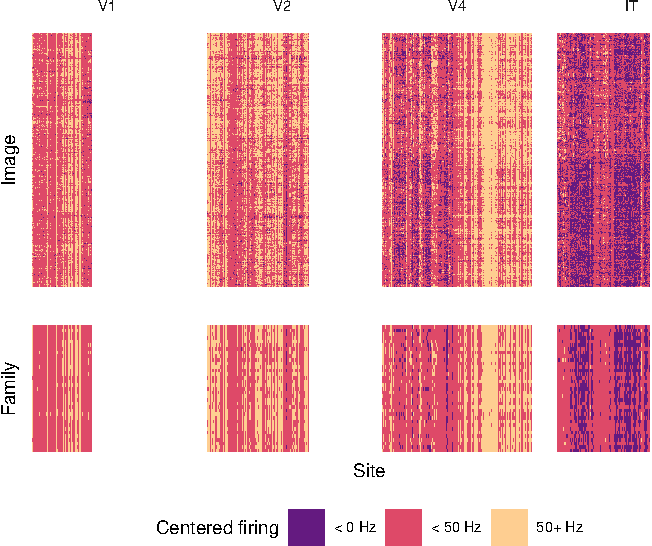
\includegraphics[keepaspectratio]{20261028_files/figure-pdf/fig-centered-1.pdf}}

}

\caption{\label{fig-centered}Heat maps of centered/baseline subtracted
firing rates, as (top) averaged over specific image repetitions or
(bottom) averaged over families. IT shows more sites with below baseline
firing. Only sites with split-half correlations \textgreater{} 0.2 are
show. See the appendix for all sites.}

\end{figure}%

\subsection{Separate sparsities for positive and negative
firings}\label{separate-sparsities-for-positive-and-negative-firings}

\begin{figure}

\centering{

\pandocbounded{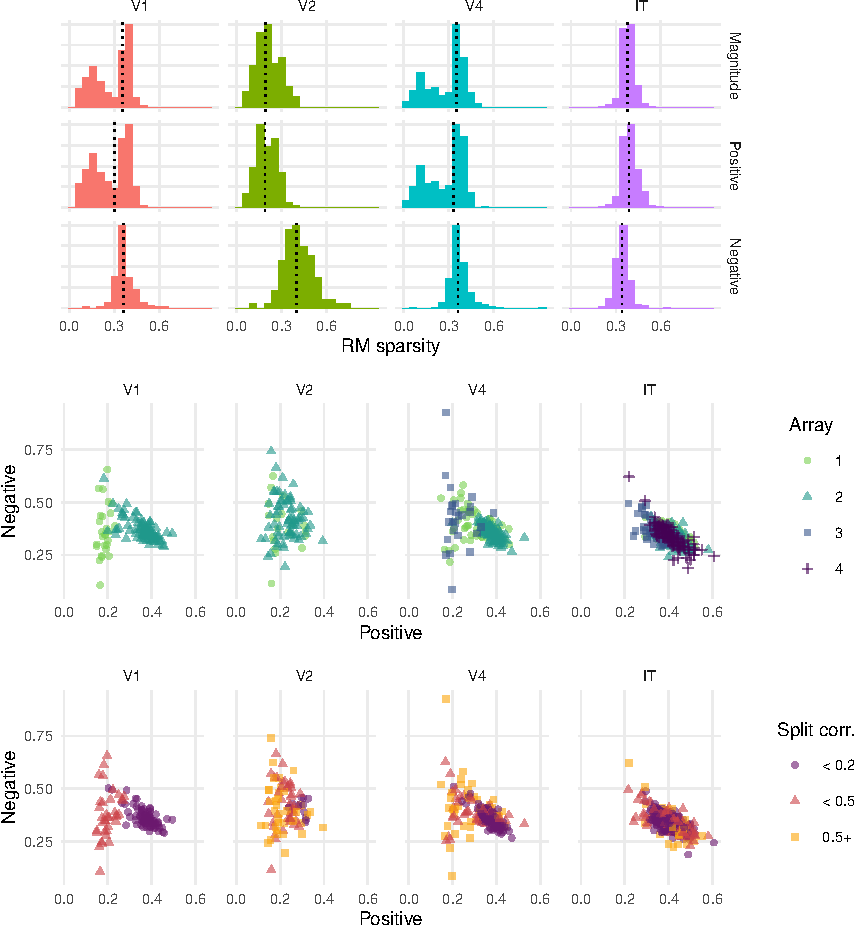
\includegraphics[keepaspectratio]{20261028_files/figure-pdf/fig-split_sparsities-1.pdf}}

}

\caption{\label{fig-split_sparsities}(Top) Histograms of site
sparsities, calculated on the absolute value of centered firing
(magnitude), only non-negative centered firing (positive), or only
negative centered firing values (negative). (Middle) For V1, V4, and IT,
each array shows distinct clusters of negative firing and positive
firing sparsity patterns. (Bottom) Labeling sites by split-half
correlation shows the same clustering.}

\end{figure}%

\section{Sparsities on log ratios}\label{sparsities-on-log-ratios}

\begin{figure}

\centering{

\pandocbounded{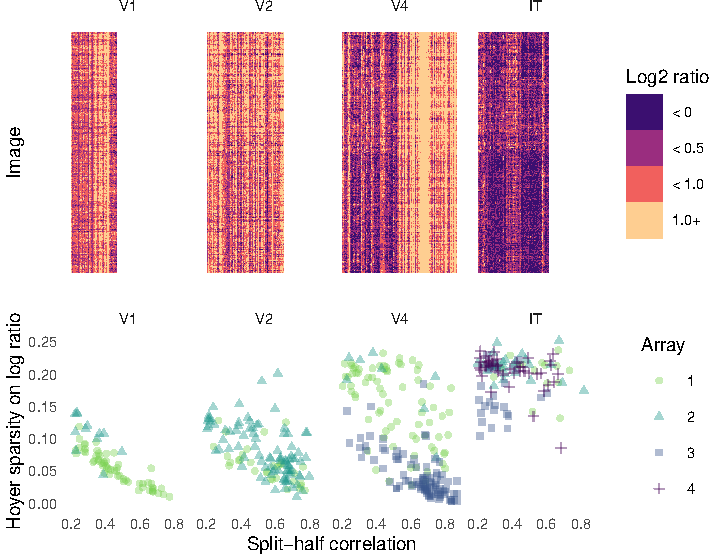
\includegraphics[keepaspectratio]{20261028_files/figure-pdf/fig-centered_lr-1.pdf}}

}

\caption{\label{fig-centered_lr}(Top) Heat maps of log (firing /
baseline), as averaged over specific image. IT shows more sites with
below baseline firing. Only sites with split-half correlations
\textgreater{} 0.2 are show. (Bottom) Scatter plots of Hoyer sparsity
vs.~reliability. Only sites with split-half correlations \textgreater{}
0.2 are show.}

\end{figure}%

\begin{figure}

\centering{

\pandocbounded{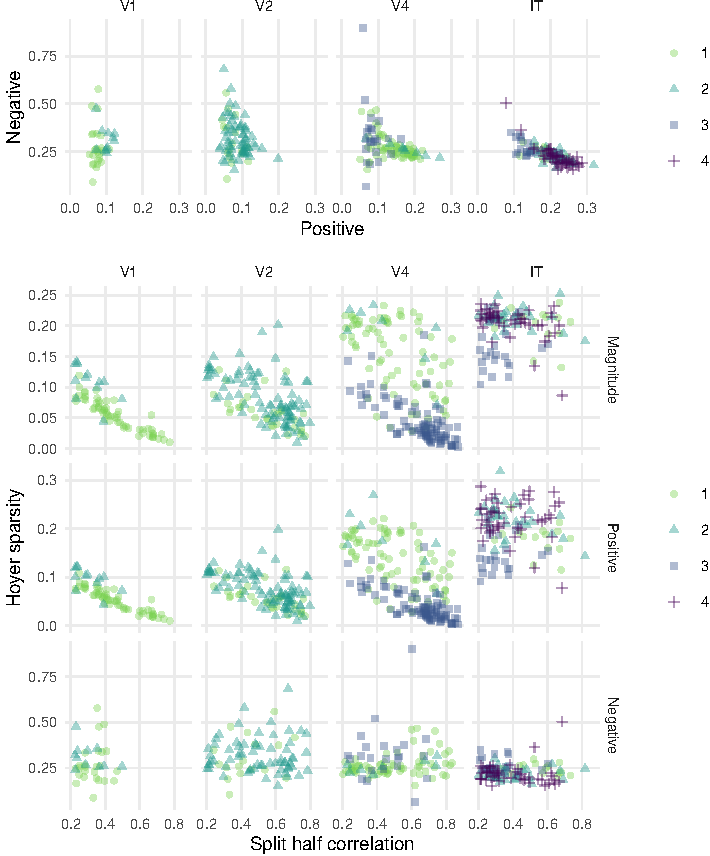
\includegraphics[keepaspectratio]{20261028_files/figure-pdf/fig-lr_split-1.pdf}}

}

\caption{\label{fig-lr_split}(Top) Scatter plots comparing sparsities
calculated on only negative vs.~only positive log ratios. (Bottom)
Sparsity vs.~correlation plots for each category of log ratios (only
negatives, only positives, all magnitudes)}

\end{figure}%

\section{Appendix}\label{appendix}

\subsection{Heat maps}\label{heat-maps}

\begin{figure}

\centering{

\pandocbounded{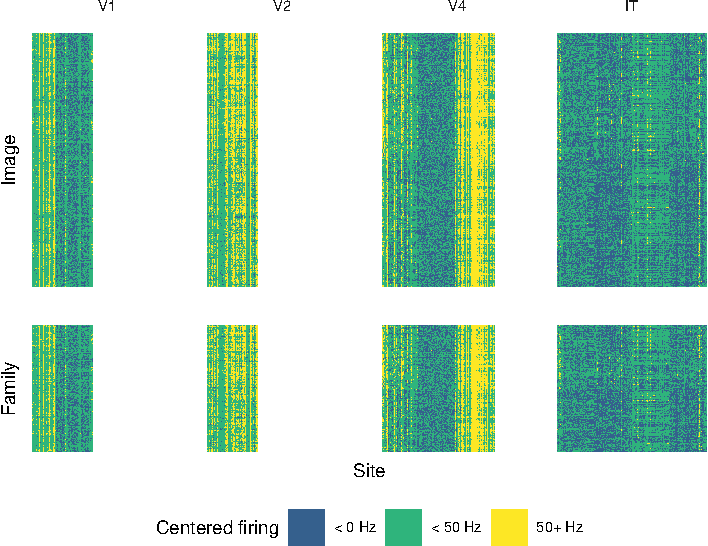
\includegraphics[keepaspectratio]{20261028_files/figure-pdf/fig-centered_full-1.pdf}}

}

\caption{\label{fig-centered_full}Heat maps of centered/baseline
subtracted firing rates, as (top) averaged over specific image
repetitions or (bottom) averaged over families. IT shows more sites with
below baseline firing.}

\end{figure}%

\subsection{Different sparsity
measures}\label{different-sparsity-measures}

\begin{figure}

\centering{

\pandocbounded{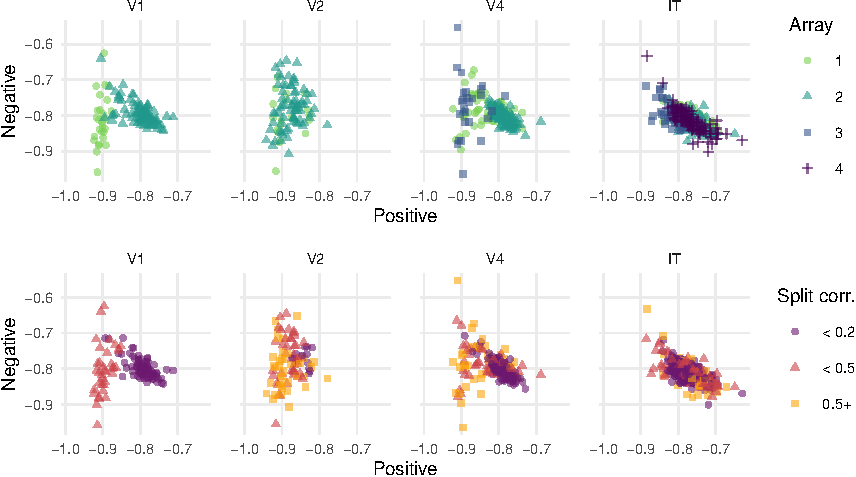
\includegraphics[keepaspectratio]{20261028_files/figure-pdf/fig-split_pq-1.pdf}}

}

\caption{\label{fig-split_pq}}

\end{figure}%

\begin{figure}

\centering{

\pandocbounded{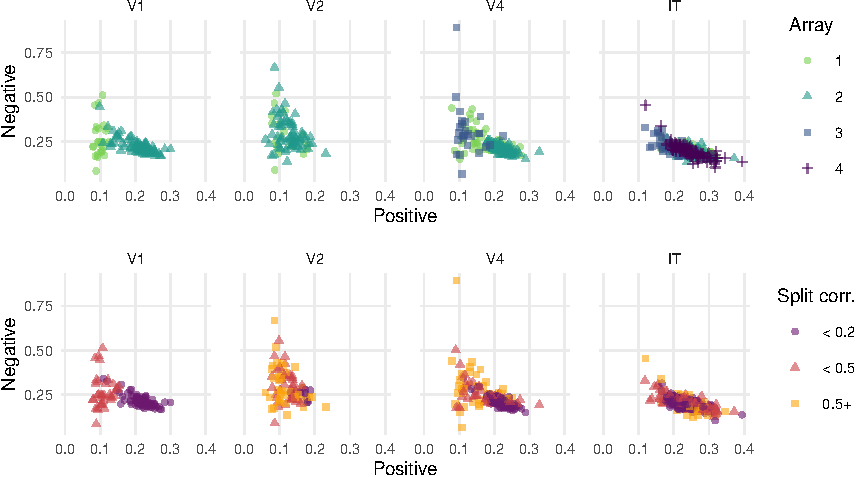
\includegraphics[keepaspectratio]{20261028_files/figure-pdf/fig-split_hoyer-1.pdf}}

}

\caption{\label{fig-split_hoyer}}

\end{figure}%

\begin{figure}

\centering{

\pandocbounded{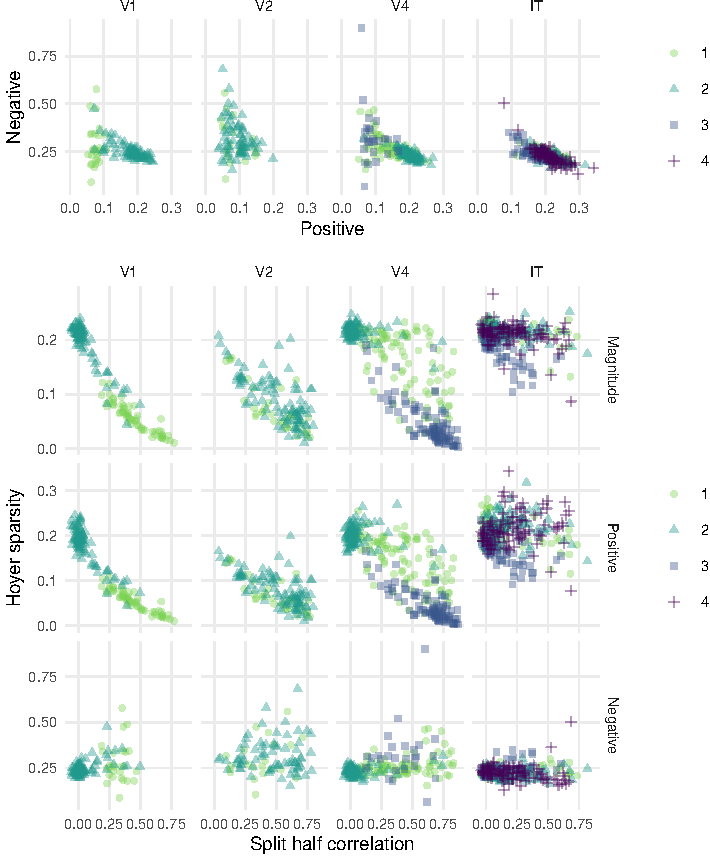
\includegraphics[keepaspectratio]{20261028_files/figure-pdf/fig-lr_split_all-1.pdf}}

}

\caption{\label{fig-lr_split_all}Same as previous figure but without
correlation cutoff.}

\end{figure}%

\subsection{Monkey details}\label{monkey-details}

\begin{longtable}[]{@{}cllll@{}}
\caption{File name codes}\tabularnewline
\toprule\noalign{}
Region & Array 1 & Array 2 & Array 3 & Array 4 \\
\midrule\noalign{}
\endfirsthead
\toprule\noalign{}
Region & Array 1 & Array 2 & Array 3 & Array 4 \\
\midrule\noalign{}
\endhead
\bottomrule\noalign{}
\endlastfoot
V1 & KY (29) & HT (36) & & \\
V2 & KY (29) & LI (29) & & \\
V4 & KY (29) & LI (29) & XT (409) & \\
IT & BB (20) & HT (34) & HU (34) & HT (221) \\
\end{longtable}

\begin{longtable}[]{@{}cllll@{}}
\caption{Codes corresponding to Table 1 in Lee et al.~}\tabularnewline
\toprule\noalign{}
Region & Array 1 & Array 2 & Array 3 & Array 4 \\
\midrule\noalign{}
\endfirsthead
\toprule\noalign{}
Region & Array 1 & Array 2 & Array 3 & Array 4 \\
\midrule\noalign{}
\endhead
\bottomrule\noalign{}
\endlastfoot
V1 & M1 (29) & M6 (36) & & \\
V2 & M1 (29) & M2 (29) & & \\
V4 & M1 (29) & M2 (29) & M8 (409) & \\
IT & M3 (20) & M6 (34) & M7 (34) & M6 (221) \\
\end{longtable}

\begin{figure}

\centering{

\pandocbounded{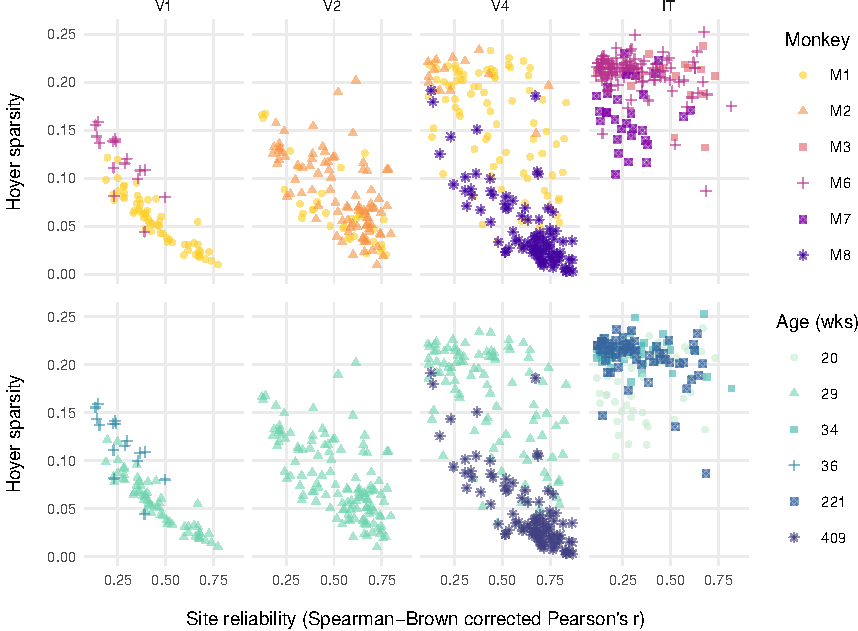
\includegraphics[keepaspectratio]{20261028_files/figure-pdf/fig-monkey-1.pdf}}

}

\caption{\label{fig-monkey}Labeling by monkey rather than array.}

\end{figure}%




\end{document}
